% !TEX root = thesis.tex

\section{Alguns invariants algebràics}\label{sec:Invariantsalgebraics}

El Teorema \ref{teo:teoremadeReidemeister} dona un mètode per saber quan dos nusos son equivalents, aquest resultat però no permet distingir quan dos nusos son diferents. D'aquesta manera per exemple, encara no sabem que $\ovoid\neq 3_1$. Per això és necessari la creació d'invariants que ens permetin realitzar aquesta tasca.\\

Recordem que un invariant és un objecte ben definit, ja sigui un número, polinomi, grup, etcètera; que podem associar a un nus qualsevol, de manera que si tenim dos nusos amb diferent valor per aquest invariant, llavors segur que els dos nusos son diferents.

\subsection{L'Ordre}\label{sec:ordrecomainvariant}

Com ja podriem haver esperat, l'ordre d'un nus és un exemple d'invariant. Nusos amb diferent ordre no poden ser equivalents. Aquest invariant però és intractable a nivell pràctic pel fet d'haver de considerar el mínim nombre de creuaments donats tots els diagrames d'aquest.\\

\begin{proposition}
	L'ordre d'un nus és una propietat topològica.
\end{proposition}

\begin{proof}
	Sigui $K$ un nus qualsevol amb diagrama $diag(K)$. Siguin $K_1, K_2, K_3, \dots$ nusos equivalents a $K$ amb els seus respectius diagrames formats a partir de diferents transformacions de $K$ com hem definit a la Secció \ref{subsec:Moviments de Reidemeister}. D'entre aquests nusos, tenim un nus $K_k$ que té el mínim nombre de creuaments $x$. Definim $O(K)=O(K_k)=x$. Evidentment, $x=O(K_1)=O(K_2)=O(K_3)=\dots$. Ara, quan transformem el nus $K$ en un nus equivalent, com aquest està a la llista de nusos, aquest també pot ser transformat en $K_k$ on $O(K_k)=x$.
\end{proof}

\subsection{El Nombre de Desnuament}\label{sec:desnuamentcomainvariant}

\begin{definition}\label{def:desnuament}
	Diem que $u(K)$ és el \underline{nombre de desnuament} del nus $K$ si aquest és el mínim nombre de canvis en els creuaments d'un diagrama de nus necessaris per tal d'aconseguir el nus trivial. $$u(K)=\min\{u(D)|\text{D diagrama de K}\}$$
\end{definition}

El nombre de desnuament és també un invariant. Aquest però, de la mateixa manera que passa amb l'ordre és intractable a nivell pràctic. Intuïtivament, si $K$ és una corba a $S^3$, llavors $u(K)$ és el mínim nombre de vegades que $K$ ha de passar per sí mateix per aconseguir el nus trivial.

\begin{proposition}\label{prop:nombrededesnuament}
	Donat un nus $K$ qualsevol, aquest sempre pot ser desnuat, i.e. $u(K)$ és finit.
\end{proposition}

\begin{proof}
	Entenem per \textit{moviment local} un canvi en els creuaments d'un nus com en el de la Figura \ref{fig:movimentlocal} passant de sobrepassos a sotapassos o a la inversa. D'aquesta manera, recorrent $K$ d'acord amb una orientació qualsevol i fent moviments locals canviant sotapassos a sobrepassos a mesura que aquests van apareixen sense modificar els creuaments que ja haguem visitat ja ho tindriem.
\end{proof}

\begin{figure}
	\centering
	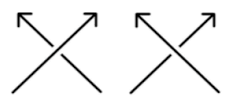
\includegraphics[width=0.6\linewidth]{img/movimentlocal.png}
	\caption{Moviments locals que es poden realitzar en qualsevol creuament d'un nus. A la imatge de l'esquerra, el tros de corda que va de  Sud-Oest fins a Nord-Est passa per sobre de la corda que el creua i doncs en aquest sentit diem que la sobrepassa. A la dreta, aquesta mateixa corda creua per sota i doncs diem que la sotapassa.}\label{fig:movimentlocal}
\end{figure}

\begin{proposition}
	Sigui $K$, $K'$ dos nusos qualssevol, llavors $u(K+K')\leq u(K)+u(K')$
\end{proposition}

\begin{proof}
	És clar que per tal de desnuar $K+K'$ només fa falta desnuar $K$ i $K'$.
\end{proof}

L'altre desigualtat és de fet un problema obert.\\

De fet, coneixer el nombre de desnuament d'un nus pot pensar-se com l'objectiu d'aquesta teoria. Si veiem que un nus $K$ no és el nus trivial i que un moviment local en algun dels creuaments dona com a resultat el nus trivial, llavors segur que $u(K)=1$. Així doncs, d'aquí a no massa estarà clar que $u(3_1)=u(4_1)=1$. No obstant, actualment encara hi ha una gran quantitat de nusos com per exemple $10_{11}$ dels quals se'ls hi desconeix el nombre de desnuament. Per aquest últim es creu que es troba entre dos i tres.\\

\subsection{El Gènere}\label{sec:generescomainvariant}

Veurem ara que tot link a $S^3$ es pot veure com la frontera d'una superfície immersa en $S^3$. Aquestes superfícies poden ser utilitzades per estudiar el link.

\begin{definition}\label{def:superficiedeseifert}
	Una \underline{superfície de Seifert} $S$ per un link $L$ orientat de $S^3$ és una superfície compacta, connexa i orientable, $S\subset S^3$ de manera que la seva frontera és $L$, i.e. $\partial S=L$.
\end{definition}

No es gens evident a partir de la Definició \ref{def:superficiedeseifert} que aquests objectes hagin d'existir i encara menys evident com es construeixen. A continuació veurem que de fet, existeix un algorisme per construir-los. Exemples d'aquestes superfícies son com les de la Figura \ref{fig:superficiedeseifert}. \\

És evident que tota superfície compacta connexa i orientada amb frontera dins $S^3$ és un exemple d'un link. Una superfície és no orientable si conté una banda de Möbius. Algunes superfícies poden ser construïdes amb un link qualsevol com a frontera de la següent manera: Pintant de color blanc i negre seguint un patró com el d'un taulell d'escacs les regions de $S^2$ que formen el complement del diagrama d'un link. Considerant totes les regions d'un mateix color i juntant-les per bandes amb una mitja volta arribem a obtenir un objecte com el de la Figura \ref{fig:trefoilseifert}.\\

\begin{figure}
	\centering
	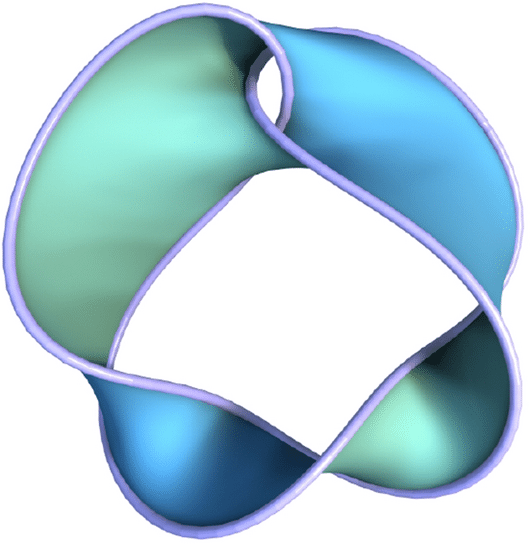
\includegraphics[width=0.6\linewidth]{img/seifertsurface.png}
	\caption{Exemple d'una superfície de Seifert per $5_2$. Framed Knots - Scientific Figure on ResearchGate.}\label{fig:superficiedeseifert}
\end{figure}

\begin{figure}
	\centering
	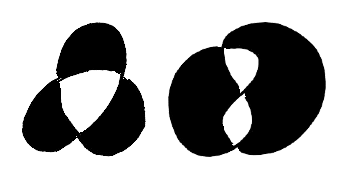
\includegraphics[width=0.6\linewidth]{img/trefoilseifert.png}
	\caption{Dos diagrames del nus $3_1$ pintats com indiquen les instruccions. Com es pot observar, la superfície de l'esquerra és no orientable al ser una cinta de Möbius amb tres mitjes voltes, la de la dreta, en canvi, sí; i doncs és una superfície de Seifert com haviem vist a la Definició \ref{def:superficiedeseifert}. Notem doncs que diagrames diferents d'un mateix nus poden o no donar lloc a una superfície de Seifert.}\label{fig:trefoilseifert}
\end{figure}

Tot i que aquest mètode pot donar com a resultat una superfície de Seifert, en general aquest no té perquè ser el cas. Herbert Seifert demostrà l'existència d'aquests objectes i donà un algorisme --- que duu el seu mateix nom --- per trobar-les [\cite{seifert}].

\begin{theorem}\label{theo:existenciadesuperficiesdeseifert}
	Tot link orientat $L$ a $S^3$ té una superfície de Seifert.
\end{theorem}

\begin{proof}
	Sigui $diag(L)$ un diagrama orientat de $L$ qualsevol i sigui $\widehat{diag(L)}$ aquest darrer diagrama modificat segons indica la Figura \ref{fig:movimentsdeseifert}, llavors $\widehat{diag(L)}$ és el mateix que $diag(L)$ excepte en un entorn prou petit de cada creuament on aquest ha sigut eliminat de la única manera coherent amb l'orientació del nus. Aquest $\widehat{diag(L)}$ és doncs una unió disjunta de corbes orientades simples i tancades dins $S^2$. D'aquesta manera, $\widehat{diag(L)}$ és la frontera de la unió d'un nombre de discs disjunts. Considerant que aquests disc es troben al mateix nivell, excepte si aquests estan un contingut en l'altre --- en aquest cas el disc de dins es considerarà a sobre l'altre disc --- juntem els discs mitjançant bandes amb una mitja volta als mateixos llocs on hi havia els creuaments. Això forma una superfície orientada amb $L$ com a frontera. Cada disc rep la orientació induïda per $\widehat{diag(L)}$ i les bandes que uneixen els diferents discos van alternant aquesta orientació.
\end{proof}

\begin{figure}
	\centering
	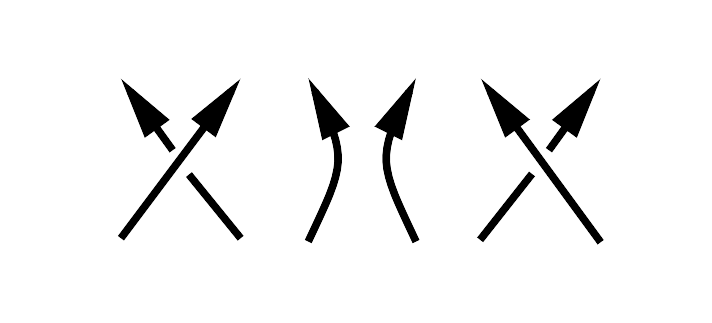
\includegraphics[width=0.6\linewidth]{img/seifert.png}
	\caption{Moviments utilitzats en l'algorisme de Seifert. Quan ens trobem amb un creuament, resoldrem aquest com mostra la imatge central reseguint el nus o link com indica la seva orientació.}\label{fig:movimentsdeseifert}
\end{figure}

En la demostració del Teorema \ref{theo:existenciadesuperficiesdeseifert}, $\widehat{diag(L)}$ era una col·lecció disjunta de corbes simples i tancades construïdes a partir de $diag(L)$. Aquestes corbes s'anomemen \underline{cercles de Seifert} del $diag(L)$. La Figura \ref{fig:cerclesdeseifert} dona un exemple d'aquesta.\\

\begin{figure}
	\centering
	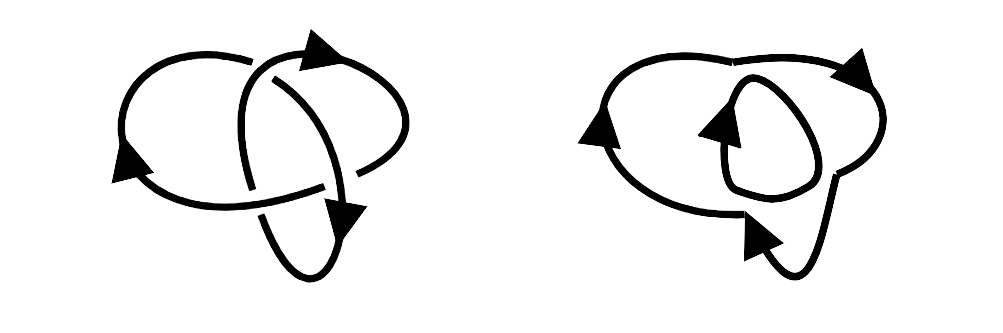
\includegraphics[width=\linewidth]{img/cerclesdeseifert.png}
	\caption{Exemple amb la construcció de $\widehat{diag(3_1)}$ a partir d'un diagrama de $3_1$ qualsevol.}\label{fig:cerclesdeseifert}
\end{figure}

Una superfície de Seifert per la Figura \ref{fig:cerclesdeseifert} s'aconsegueix superposant els dos cercles de Seifert disjunts un a sobre l'altra i unint-los mitjançant tres bandes amb una mitja volta cadascuna en els creuaments. Evidentment, com hem vist a la demostració aquest algorisme dona lloc a una superfície de Seifert. Donat un diagrama qualsevol de $L$ però, aquesta no té perquè ser única. Tampoc té perquè ser la més senzilla donat un diagrama qualsevol.

\begin{figure}
	\centering
	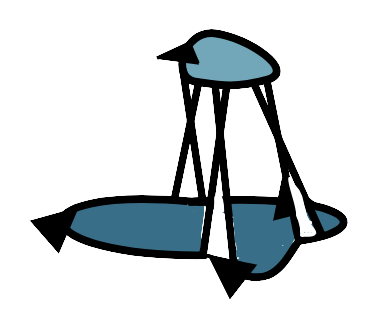
\includegraphics[width=0.6\linewidth]{img/superficiedeseifert.png}
	\caption{superfície de Seifert pel nus $3_1$ obtinguda unint els discos a través de bandes amb una mitja volta. Una senzilla comprovació demostra que la frontera de la superfície és el mateix nus.}\label{fig:superficiedeseifert2}
\end{figure}

\begin{definition}\label{def:genere}
	El \underline{gènere} $g(K)$ d'un nus $K$ es defineix com $$g(K)=\min\{g(S)| \text{S superfície de S. de K}\}$$ Direm que una superfície de Seifert $S$ amb $K$ com a frontera és \textit{minimal} si $g(S)=g(K)$.
\end{definition}

\begin{proposition}
	El gènere d'un nus és una propietat topològica.
\end{proposition}

\begin{proof}
	Considerem una superfície de Seifert minimal $S$ que té per frontera $K$. Com $K$ és equivalent a $K'$ llavors ha d'existir un homeomorfisme $h:S^3\rightarrow S^3$ de manera que $h(K)=K'$. Llavors, $h(S)$ és una superfície de Seifert que té per frontera $K'$ i $g(h(S))=g(S)=g(K)$. A més, $h(S)$ és una superfície de Seifert minimal que té $S'$ per frontera i per tant $g(K)=g(K')$. Si $h(S)$ no fos una superfície de Seifert minimal de $K'$, llavors existiria una superfície de Seifert minimal $S'$ que tindria $K'$ per frontera i tal que $g(S')<g(h(S))$ i per tant $h^{-1}(S')$ seria una superfície de Seifert amb $K$ per frontera amb gènere menor que $g(S)$, però això no pot ser ja que $S$ és minimal.
\end{proof}

Com en aquest cas $K$ és un nus, $S$ només té una component de frontera de manera que com a superfície abstracta és un disc amb un nombre concret de "mànecs". A aquest nombre se l'anomena gènere. Més precisament, el gènere de $S$ és

\begin{equation}\label{eq:generedunasuperficie}
	g(S)=\frac{1}{2}(1-\mathcal{\chi}(S))
\end{equation}

on $\mathcal{\chi}$ és la característica d'Euler de $S$. La característica d'Euler es pot definir paral·lelament com el nombre de vèrtex menys el nombre de costats més el nombre de triangles en qualsevol triangulació de $S$.\\

Si $diag(K)$ té $n$ creuament i $s$ cercles de Seifert, llavors $\mathcal{\chi}(S)=s-n$ de manera que

\begin{equation}\label{eq:cotasuperiorgenere}
	g(K)\leq \frac{1}{2}(n-s+1)
\end{equation}

Aquest invariant té un millor tractament que els vistos anteriorment. Donem ara una caracterització del nus trivial en termes del gènere.

\begin{proposition}
	$K$ és el nus trivial si i només si $g(K)=0$.
\end{proposition}

\begin{proof}
	Si $K$ és el nus trivial, llavors un disc amb frontera $K$ és clarament una superfície de Seifert minimal amb $K$ per frontera. I com que un disc és una esfera amb un component de frontera deduïm que $g(K)=g(S^2)=0$. Alternativament, si $K$ és tal que $g(K)=0$, llavors existeix una superfície de Seifert minimal $S$ amb $g(S)=0$, d'aquesta manera $S$ és una esfera amb una component per frontera, i.e. un disc.
\end{proof}

Seguint amb l'exemple del nus $3_1$, llavors es veu clarament que $g(3_1)=1$. Per tant, deduïm que $3_1\neq\ovoid$. De manera similar un pot arribar a calcular els gèneres d'un gran nombre de nusos. El problema amb aquest mètode és que l'Equació \ref{eq:cotasuperiorgenere} dona una cota superior per aquest gènere i per tant, a mesura que incrementem el nombre de creuaments és possible que el gènere pugui prendre un nombre finit de valors diferents entre ells. Per exemple, un exercici senzill demostra que $g(8_{20})\leq2$ i doncs pot ser 1 o bé 2.

\subsubsection{Additivitat i aplicacions}

\begin{theorem}\label{teo:sumabilitatdelgenere}
	Donats dos nusos $K$ i $K'$, $$g(K+K')=g(K)+g(K')$$
\end{theorem}

\begin{proof}
	Comencem veient $g(K+K')\leq g(K)+g(K')$. Considerem que $K$ i $K'$ estan separats per un pla i considerem les superfícies de Seifert minimals de tots dos nusos $S$ i $S'$ ($S$ i $S'$ també estan separades pel pla). Donem una orientació a $K$ i $K'$ i considerem la seva suma assegurant-nos que $K+K'$ no intersecti $Int(S)$ ni $Int(S')$. Considerem ara una banda $B$ que conecta $K$ i $K'$ que té per frontera els dos segments de corda introduïts al considerar la suma $K+K'$ i de tal manera que $B$ no intersecta $Int(S)$ ni $Int(S')$. D'aquesta manera, $B$ conecta $S$ i $S'$ i doncs $C=S\cup S'\cup B$ és una superfície de Seifert per $K+K'$. Finalment com $g(C)=g(S)+g(S')=g(K)+g(K')$ tenim $g(K+K')\leq g(K)+g(K')$. L'altre desigualtat es pot trobar a \cite{rolfsen2003knots}.
\end{proof}

A partir del Teorema \ref{teo:sumabilitatdelgenere} obtenim un seguit de resultats:

\begin{corolary}
	Cap nus tret del nus trivial té oposat respecte la suma. És a dir, que si $K+K'=\ovoid$, llavors $K=K'=\ovoid$.
\end{corolary}

\begin{proof}
	Suposem que existeix $K$ i $K'$ amb almenys un d'ells diferent del nus trivial de manera que $K+K'=\ovoid$, llavors en virtut del Teorema \ref{teo:sumabilitatdelgenere}
	\begin{align*}
		&g(K+K')=g(K)+g(K')\\
		&0=g(K)+g(K')
	\end{align*}
	Com que el gènere d'un nus és un nombre positiu, tenim que $g(K)=g(K')=0$.
\end{proof}

\begin{corolary}
	Hi ha un nombre infinit de nusos diferents.
\end{corolary}

\begin{proof}
	Sigui $K$ un nus no trivial qualsevol i $\sum^{n}K$ la suma de $n$ còpies d'aquest. Veiem que si $n\neq m$, llavors $\sum^{n}K\neq\sum^{m}K$. Suposem que $\sum^{n}K=\sum^{m}K$, aleshores $\sum^{n}g(K)=\sum^{m}g(K)$. Sense pèrdua de generalitat podem suposar que $m>n$, d'aquesta manera $\sum^{m-n}g(K)=0$ cosa que implica $K=\ovoid$. Contradicció amb el fet que $K$ no pot ser trivial.
\end{proof}

\begin{corolary}
	Un nus $K$ amb gènere $1$ és primer.
\end{corolary}

\begin{proof}
	Sigui $K$ un nus amb $g(K)=1$ i expressem aquest com a suma de nusos $K_1$ i $K_2$, llavors $1=g(K_1)+g(K_2)$ i per tant $g(K_1)=0$ o al revés.
\end{proof}

\begin{corolary}
	Tot nus $K$ pot ser expressat com a suma finita de nusos primers.
\end{corolary}

\begin{proof}
	Si $K$ és primer, llavors el resultat és obvi. Suposem ara que $K$ no sigui un nus primer. Per definició, existeixen $K_1$ i $K_2$ tots dos diferents del nus trivial de manera que $K=K_1+K_2$ i del Teorema \ref{teo:sumabilitatdelgenere} sabem que $g(K_1),g(K_2)<g(K)$. Ara, fent el mateix procés amb $K_1$ i $K_2$ podem concloure que $K$ és suma de nusos primers.
\end{proof}

\begin{corolary}
	Existeixen nusos amb un nombre de creuaments arbitràriament gran.
\end{corolary}

\begin{proof}
	Sigui $K$ un nus qualsevol, com que el nombre de cercles de Seifert sempre serà com a mínim $1$, utilitzant l'Equació \ref{eq:cotasuperiorgenere} tenim $$g(K)\leq \frac{n}{2}$$ on $n$ és el nombre de creuaments del diagrama de $K$. Considerem ara un nus no trivial i $K_m=\sum^{m}K$ la suma de $m$ còpies de $K$. Llavors, $$m\leq g(K_m)\leq \frac{c(K_m)}{2}$$ on $c(K_m)$ és el nombre de creuaments de la suprfície de Seifert de $K_m$. A mesura que $m$ s'acosta a infinit, també ho fa $c(K_m)$.
\end{proof}

Cal remarcar que existeixen cotes inferiors pel gènere d'un nus qualsevol [\cite{lowerbound}] i que hi ha classes de nusos amb molt bones propietats pel que fa el seu gènere. Nosaltres però, ens limitarem a fer-ne menció i classificarem els nusos d'ordre més baix utilitzant només els resultats vistos.\\

La Figura \ref{fig:genus} mostra una taula per al gènere d'un nus primer de fins a $7$ creuaments.

\begin{figure}
	\centering
	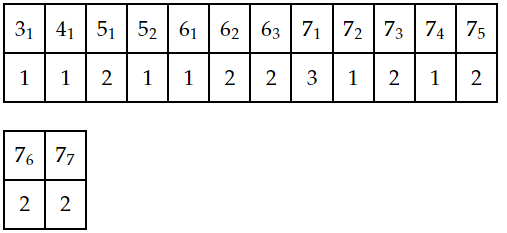
\includegraphics[width=\linewidth]{img/genus.png}
	\caption{Gènere de tots dels nusos primers de fins a $7$ creuaments.}\label{fig:genus}
\end{figure}